\documentclass[Report.tex]{subfiles}
\begin{document}

\chapter{Implementation}
The details of each component of the project are discussed in this chapter. A large proportion of this project concerned the retrieval and manipulation of data from various sources. Refining the input to the APIs and databases resulted in higher success rates of the queries, the creation of more informative datasets, and improved representation of data on the client side. The process of improving these aspects was iterative, and each modification was tested to assess whether the change in output had a positive effect. The key developments in geocoding, querying the MySQL database for concepts, and ordering the concepts are discussed in the current chapter.

\section{The Python Programming Language}
\subsection{Language Features}
Python is a dynamically typed, multi-paradigm language with an extensive package system outside of the standard library \cite{pythonabout}.  It was chosen due to its ease of use and applicability for a wide variety of relevant tasks, including HTTP request handling, unit testing and JSON object encoding/decoding. Throughout this project, I have found these and modules such as \texttt{subprocess} for spawning a MetaMap process, and external libraries such as BioPython for submitting Entrez requests, extremely useful for the tasks at hand. This is the greatest strength of Python - if a tool has not already been made by the active community of developers, it is possible (and encouraged) for one to build a new library themselves.

\subsection{The Flask Microframework}
Flask is an extremely lightweight web framework (available at \url{http://flask.pocoo.org/}), requiring minimal input to produce a basic server that can route requests from the client. This was perfect for the simplicity of the application, that currently does not require user or admin accounts and the associated security risks and storage implications. Though a cache was eventually implemented, this is external to the core of the framework as all input comes from the backend.

\subsection{Project Structure}
\noindent That Python programs do not explicitly require a structure is one of its strengths - but also a potential downfall for inexperienced developers. Modules can be organised into packages with the inclusion of a \texttt{\_\_init\_\_.py} file, but even this is optional. It was difficult to know how to structure the application, particularly with the usage of the Flask microframework . However with the popularity of MVC-like frameworks such as Django and Ruby on Rails it was not difficult to find comparable projects to base the directory structure of the application on. It is also largely down to the personal preference of the developer, and does not impact the performance of the application at all. Within modules, there is a choice to be made between keeping the module as a collection as functions, or turning it into a Class to utilise object-orientated programming principles and patterns. In a language such as Java or Ruby, I most likely would have created a Citation class with attributes for important fields such as PMIDs, and written getters for each. In Python, this style of programming is possible but perhaps overwrought considering the ease with which Python handles JSON objects and decodes them into dicts. Each PubMed entry has a large number of fields, so would have required complicated objects (with a number of fields set to null, as few elements are mandatory) to fully represent all citation types. Citation objects were left as JSON objects/Python dicts to decrease the overhead of object creation, and also to simplify the passing of messages between modules, at the cost of a better defined structure.\newline
 
\noindent In Chapter 2, the general pipeline was described. Figure \ref{fig:sequence} shows in finer detail the order of the function calls from the \texttt{controller} module. The lifelines in sequence diagrams usually represent the creation and destruction of objects, however Object-Orientated programming was not used in this project. Therefore it can be assumed that the modules are only in use whilst the function calls are being carried out.\newline

\begin{figure}[ht!]
\begin{center}
\includegraphics[width=0.9\textwidth]{../lib/images/sequence.png}
\caption{Schematic of the key processes of the system, as explained in the text.}
\label{fig:sequence}
\end{center}
\end{figure}

\section{Retrieving Citations From PubMed}
As mentioned above, BioPython was used as an intermediary library between this application and the NCBI E-Utils. This was not strictly necessary, as the E-Utils are accessible via simple HTTP requests. However, BioPython automates many of the finer tunings, ensuring that the query rate is not greater than 3 per second (source code available at \url{https://github.com/biopython/biopython/blob/master/Bio/Entrez/} and documentation at \url{http://biopython.org/DIST/docs/api/}). First, the search term is sent as an argument parameter to the eSearch utility. This returns a list of up to 100,000 relevant PubMed IDs, limited to 20 for this application \cite{eutils-indepth}. This list is then sent to the eFetch utility to retrieve full PubMed records for all 20 papers.\newpage

\section{Searching For Concepts Using MetaMap}
\subsection{The Utility of MetaMap}
Due to the problems of Word-Sense Disambiguation in natural language processing, it was assumed that directly searching the UMLS for concepts would not have a high success rate. For example, a title such as \emph{"Loss of SMAD4 Promotes Colorectal Cancer Progression by Accumulation of Myeloid-Derived Suppressor Cells through CCL15-CCR1 Chemokine Axis"} contains composite phrases e.g. "cancer progression" that confer additional information together as opposed to when processed separately. This semantic analysis is would be challenging to implement manually and would most likely result in inaccuracies.

\subsection{MetaMap vs. The MTI}
\noindent MetaMap can be invoked either locally or via the Semantic Knowledge Representation Web API within the MTI. Both options were tested to compare performance. The MTI results are more refined (see Table \ref{tab:mm-results}), and consequently produce concept visualisations that are easier to understand (Figure \ref{fig:mm-screen}). Compared to the visualisation in Figure \ref{fig:screen1} produced using the MTI, there are more nodes, and many co-occur in the same hierarchies, suggesting some data redundancy. In Table \ref{tab:mm-results} it can be seen that MetaMap alone produced a higher number of results, some of which were inaccurate. For example, the phrase \emph{"Chemokine Axis"} appears to have been incorrectly interpreted by MetaMap to consist of two separate terms, resulting in the concept \emph{"Axis vertebra"} (MetaMap, concept 2). Results from the MTI are a better fit for this project, however the performance difference is not trivial if the application is run single-threaded. On a standard broadband connection, the full MTI process takes around 5-10 minutes. This is in contrast to running MetaMap locally, the output of which is delivered after less than a minute. As detailed in the next chapter, using the Python module \texttt{concurrent.futures} enabled parallelisation of most of the core processes of the application, so that there is no performance benefit to using MetaMap run locally. For these reasons, the MTI was a superior option for discovering concepts in citations. \newline

\begin{table}[!ht]
\begin{center}
    \begin{tabular}{ | c | l | l | }\hline
    \textbf{\#} & \textbf{MTI concepts} & \textbf{MetaMap concepts}\\ \hline
1 & CCL15 protein, human & Axis\\ \hline
2 & \*Macrophage Inflammatory Proteins & Axis vertebra\\ \hline
3 & \*Chemokines, CC & chemokine\\ \hline
4 & \*Chemokines & Disease Progression\\ \hline
5 & \*Colorectal Cancer & CCL15 protein, human\\ \hline
6 & \*Disease Progression & Genus Axis\\ \hline
7 & \*Neoplastic Processes & Promotion (action)\\ \hline
8 & \*Neoplasms & Loss\\ \hline
9 & Receptors, CCR1 & Progression\\ \hline
10 & \*Antigen Presentation & CCL15 gene\\ \hline
11 & immunology & CCR1 gene\\ \hline
12 & - & Chemokine (C-C Motif) Receptor 1\\ \hline
13 & - & SMAD4 gene\\ \hline
14 & - & Cancer Genus\\ \hline
15 & - & Cells\\ \hline
16 & - & Cells [Chemical/Ingredient]\\ \hline
17 & - & Colorectal\\ \hline
18 & - & Derivation\\ \hline
19 & - & Derived value\\ \hline
20 & - & Malignant Neoplasms\\ \hline
21 & - & Myeloid\\ \hline
22 & - & Primary malignant neoplasm\\ \hline
23 & - & Suppressor\\ \hline
24 & - & Suppressor Device Component\\ \hline
    \end{tabular}\\
    \caption{Output from MetaMap and MTI for the title \emph{"Loss of SMAD4 Promotes Colorectal Cancer Progression by Accumulation of Myeloid-Derived Suppressor Cells through CCL15-CCR1 Chemokine Axis"}.}
\label{tab:mm-results}
\end{center}
\end{table}
\begin{figure}[ht!]
\begin{center}
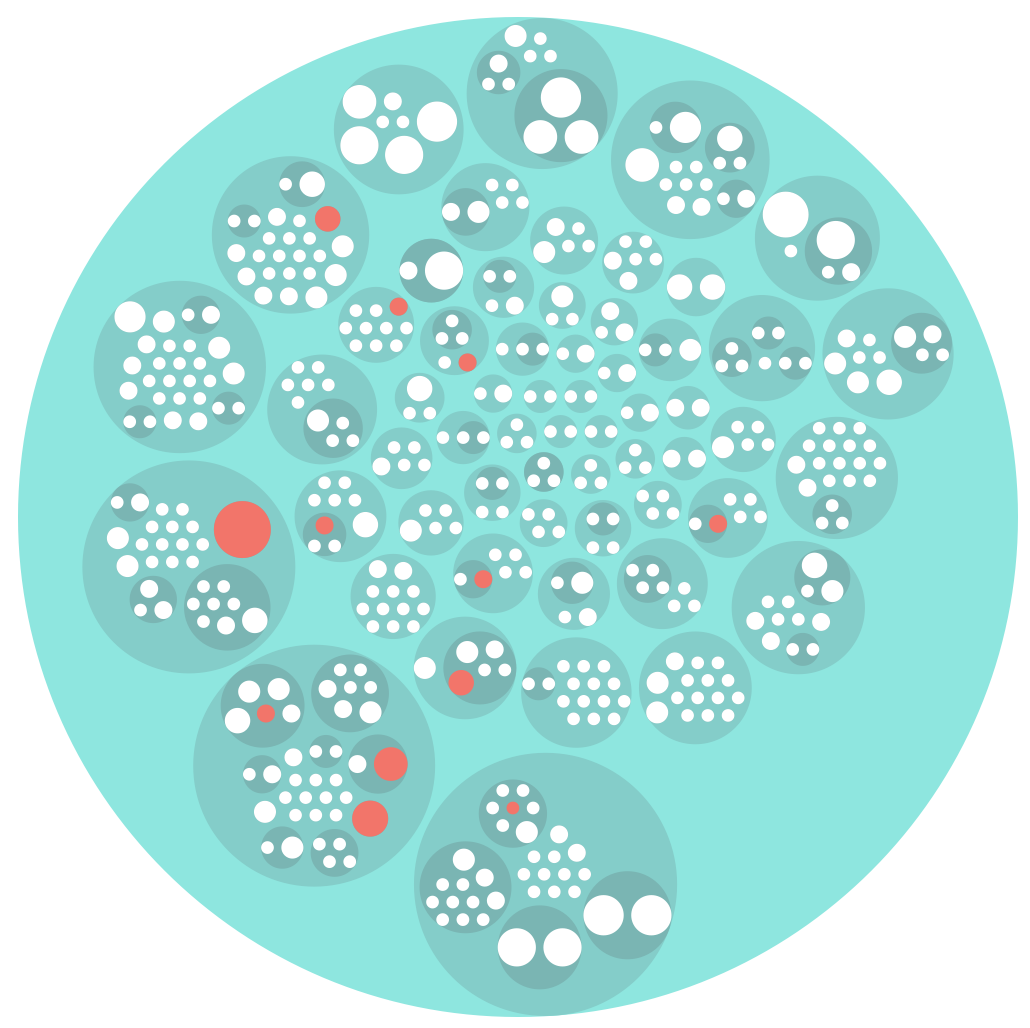
\includegraphics[width=0.4\textwidth]{../lib/images/mm-screen.png}\\
\caption{The concept visualisation from the search term 'computer' using local MetaMap.}
\label{fig:mm-screen}
\end{center}
\end{figure}

\section{Organising Concepts Into Hierarchies}
\subsection{MetaThesaurus Setup}
The MetaThesaurus is free to download from the NIH (available at \url{http://www.nlm.nih.gov/research/umls/licensedcontent/umlsknowledgesources.html}) with a valid UMLS Terminology Services account. The NIH provides database subsets for Microsoft Access, Oracle or MySQL Relational Database Management Systems. MySQL was implemented due to the proprietary nature of Access and Oracle. During installation, 70 vocabularies were chosen for inclusion based on the MetaThesaurus defaults and the language specified, which was restricted to English. These are listed in the appendix, Table \ref{tab:vocabs}. Each concept, identified by its unique concept ID (CUI), has at least one Semantic Type to inform the visualisation of gross hierarchies. To achieve a more granular representation, a direct parent is also retrieved.\newpage

\subsection{Querying MySQL}
An external library, PyMySQL, was used to execute SQL queries from the \texttt{umls} module. A summary of the database schema is shown in Figure \ref{fig:db}, showing only the attributes and tables necessary for the query. The query (listing 2 in the appendix) receives a list of CUIs as input and returns the Semantic Type (from \texttt{MRSTY}) as well as any direct parents (from \texttt{MRREL}). Direct parent concepts are defined as having a \texttt{MRREL.RELA} relationship of 'inverse\_isa'. This was chosen due to its explicit mapping of a parent/child hierarchy, and as a result of investigating similar options \texttt{MRREL.REL} = 'RB' (broader relationship) and \texttt{MRREL.REL} = 'PAR' (parent) that return results that were not true 'isa' relationships. Not all concepts have an 'inverse\_isa' relationship, and therefore outer joins were used to allow null values.\newline

\noindent Each concept is represented in multiple vocabularies, each with their own string. To standardise the nomenclature used as much as possible, only the name from highest ranked source for each CUI are returned. Rankings are defined in \texttt{MRRANK}, and the default rankings were used. The top ranking is 313, held by the MetaThesaurus preferred names (\texttt{SAB} = 'MTH', \texttt{TTY} = 'PN'). It was discovered that there are 2,295,761 CUIs in the database, of which only 172,139 have a MTH/PN source. For this reason, it was decided not to restrict just to the top ranking vocabulary as this would exclude a large proportion of the dataset. Resulting rows are also ordered by Semantic Type tree numbers (\texttt{MRSTR.STN}) before the \texttt{GROUP BY}, so that only the node furthest up the hierarchy is used as a Semantic Type.

\begin{figure}[ht!]
\begin{center}
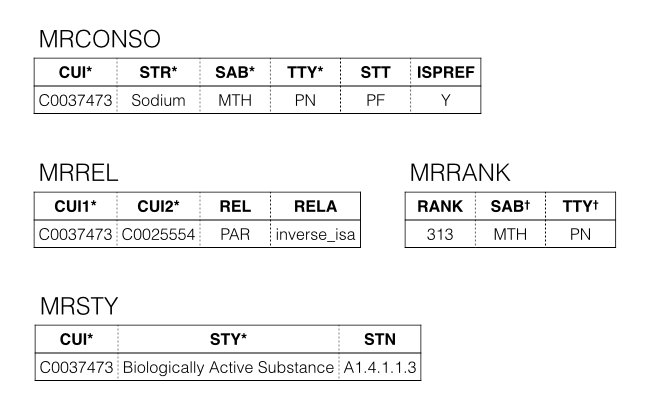
\includegraphics[width=0.7\textwidth]{../lib/images/db.png}
\caption{Fields and tables used in the SQL query to retrieve concepts, their direct parents, and their semantic types. Daggers indicate primary keys and asterisks indicate non-unique indexes. These are not necessarily exhaustive as not all fields are displayed. Multiple key fields represent composite keys. }
\label{fig:db}
\end{center}
\end{figure}

\noindent After the SQL query has produced rows corresponding to the semantic types and direct parents of all concepts, these can be formatted into nested Python dicts, ready for encoding as JSON objects for the client-side JavaScript functions. Example output from the \texttt{umls} module can be seen below. The remote MTI service was used to attain the concept IDs. There are some redundancies in data, for example both the Semantic Type and parent concept of 'computers' is 'Manufactured Object', however I think it is best to retain this structure, which may be informative if another concept also has the Semantic Type of 'Manufactured Object', but not the direct parent. Additionally, both child concepts 'Nurse' and 'Nursing Staff, Hospital' were produced, though this overlap is difficult to solve without access to the internal workings of the MTI.\newpage

\begin{verbatim}
{
  "name": "Mental Process"
  "children": [
    {
      "name": ""
      "children": [
        {
          "name": "Attitude of Health Personnel",
          "PMIDs": [ "24804813" ]
        },
        {
          "name": "Attitude to Computers",
          "PMIDs": [ "24804813" ]
        },
        {
          "name": "Computer Literacy",
          "PMIDs": [ "24804813" ]
        }
...
}
\end{verbatim}

\section{Geocoding}
\subsection{Optimisation}
The overhead of geocoding an address for the first time is high; the Text Search service in the Google Places API returns the top ten results that match the input parameters. In order to try and make the results more precise, the 'types' parameter is provided to specify that results should be either a university, a hospital, or an 'establishment' which is set as the default if a type is not present. In order to maximise the number of meaningful results achieved by the API, the input was optimised to improve the chance that a. any location is returned (from this point onward referred to as the 'hit rate'), and b. that the location returned is correct i.e. accurate. A number of formatting options were empirically tested, enabling an informed decision to be made for the geocoding function in the application.\newline

\noindent In order to have confidence in applying these findings to the larger population of papers available on PubMed, a dataset with papers on a range of topics, from various journals, and originating from numerous countries was required. Statistics on the publishing distribution between countries was found on Medline Trend \cite{medlinetrend},  though the data was limited to a date range of 2008-2012. Table \ref{tab:countries} in the appendix lists the ten countries with the most papers, their percentage share and the corresponding number of papers used in the dataset. Each of the ten countries with the most papers is represented at least once in the dataset, listed in table \ref{tab:dataset} in the appendix. 33 unique papers and 178 addresses were included to assess the hit rate, and 10 papers and 18 addresses were included to assess the accuracy. Expected locations were found manually using the Google Maps website, and therefore were tested at a smaller scale. The distance between the 'true' location and the geographical coordinates as returned by Text Search could then be compared. A radius of 5 kilometres was chosen as the cut-off distance for a location to be called as accurate. It is important to note that the allocation of correct addresses was somewhat subjective. Automation would have been preferred, however it was not possible to retrieve papers with exclusively the affiliation address in the query. Even if this could have been achieved, universities with campuses distributed over a large area may have produced misleading conclusions.\newline

\noindent A number of formatting combinations were tested, as detailed in Figure \ref{fig:geoscatter}. As expected, there was an inverse correlation between the hit rate and the accuracy of geocoding; sending more information (a higher number of address lines, particularly at the start of the address) reduces the chance of a match to a location, however the location is more likely to be correct.\newline

\noindent The first optimisations were carried out after observing trends during development. Email addresses of the lead author are sometimes included at the end of their affiliation address, which appeared to obfuscate the address for the Text Search service. Regular expressions were implemented from the \texttt{re} Python module in order to remove strings that matched the expected pattern for emails. As can be seen in Figure \ref{fig:geoscatter} (points 0 \& 1), removing email addresses did improve the hit rate of geocoding by 1\%. Of 15 addresses that contained email addresses, one (the Chinese Academy of Agricultural Sciences in Beijing) was matched to a location before removal of the email address. After formatting to remove the email address, 3 additional addresses were successfully matched to a location, however the Beijing address could not be matched. By checking the coordinates of the original returned address, it appears that the geocoding algorithm incorporated the email string to match the address to the Natural History Museum in London. In the accuracy dataset, 3 addresses included an email address but the hit rate was zero both before and after removal of the email address. From the incongruous result seen in the hit rate data, a tentative conclusion can be drawn that removing the email address improves the accuracy of results, though by a nominal amount. Spurious data was also seen elsewhere in the dataset, indicating that the input query can only be optimised to a certain degree.

\begin{figure}[!ht]
\begin{center}
	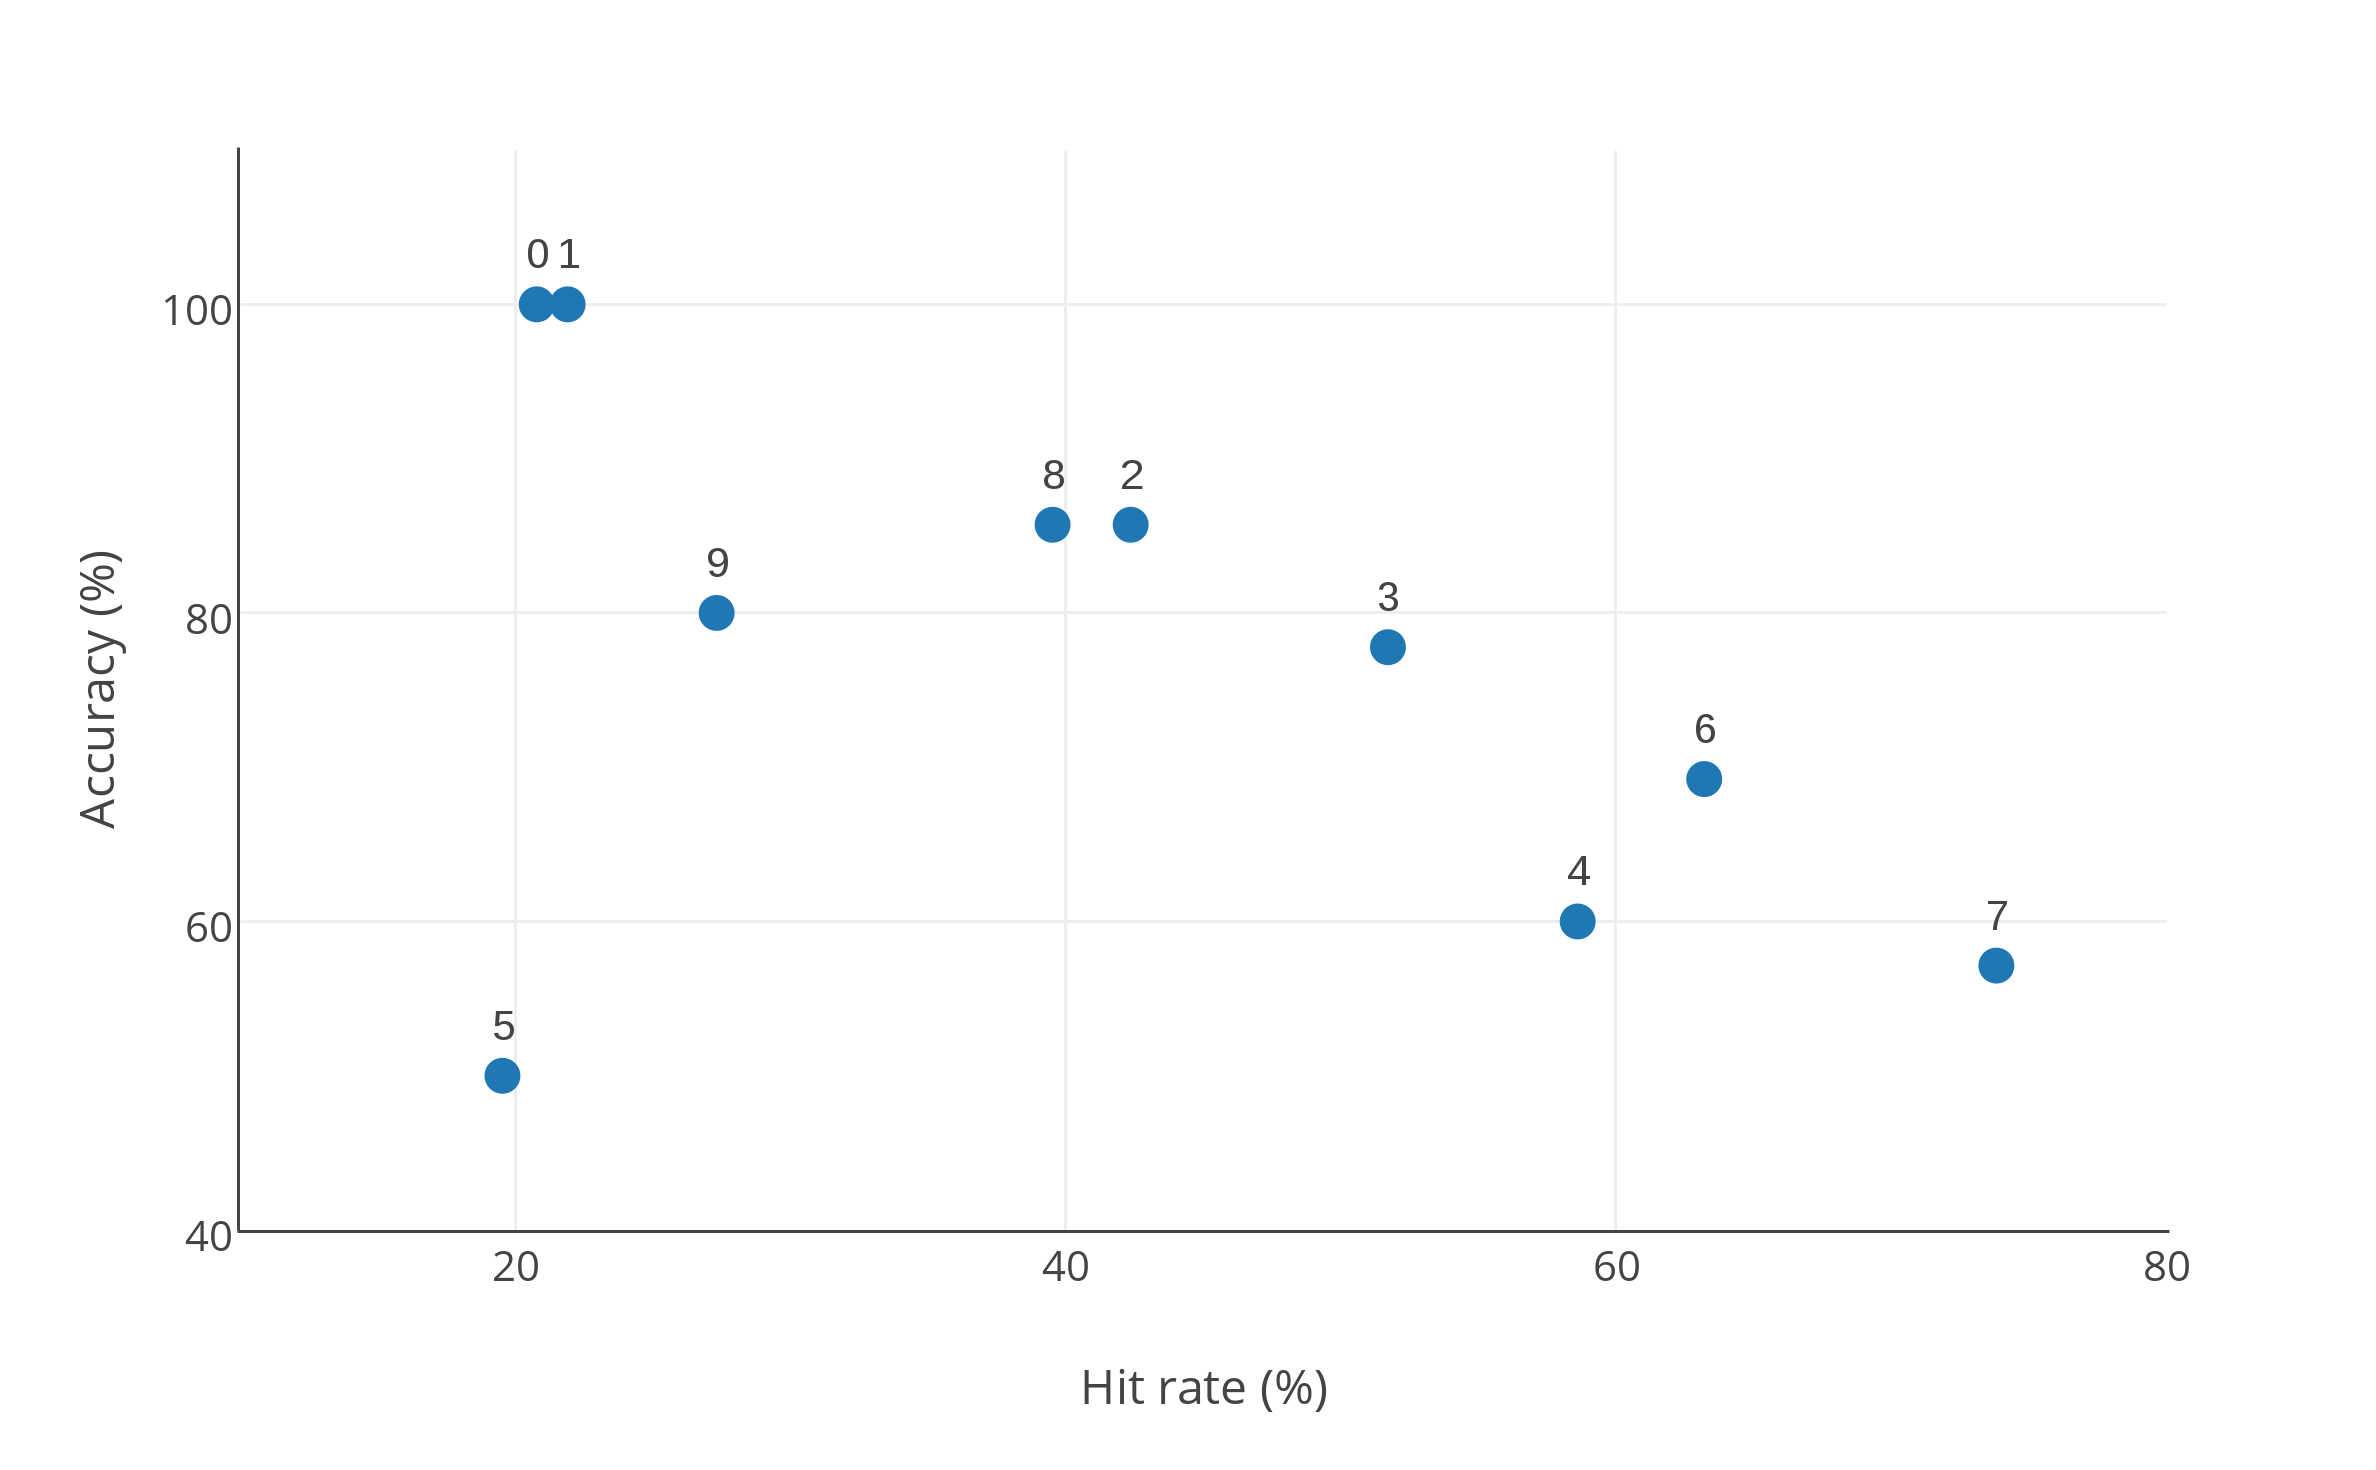
\includegraphics[width=0.8\textwidth]{../lib/images/geocode_performance_scatter}
	\caption{The hit rate (proportion of searches that returned any result, x-axis) and accuracy (proportion of searches that returned a result within 5 km of the expected location, y-axis) of 10 formatting options are plotted on this graph. The numbered points represent the following formats: 0 - none, 1 - email addresses removed, 2 - department removed, 3 - first line removed, 4 - department and first line removed, 5 - last 2 lines only, 6 - second and third lines only, 7 - second and last lines only, 8 - last 3 lines only, 9 - first 2 lines removed. Only options 0 and 1 include all addresses, as they are not limited by the number of lines in an address. \label{fig:geoscatter}}
\end{center}
\end{figure}
\newpage

\noindent Removing lines with 'department' or 'dept' was compared to an uninformed removal of the first line, and then the two approaches were combined (Figure \ref{fig:geoscatter}, points 2, 3 \& 4 respectively). Removing the first line gave the best compromise between a reduced hit rate but increased accuracy, so this approach was adopted in later formats. Sending the last two lines of each address (Figure \ref{fig:geoscatter}, point 5) resulted in a low hit rate and low accuracy results, most likely due to the number of lines averaging around 4 (see the appendix, Figure \ref{fig:addresslines}), resulting in addresses that only specify the region and the country. It was surprising to see that the Places API would not geocode areas such as 'TN, USA', perhaps to focus on matching addresses as the primary use case of the service.\newline

\noindent After taking into account the data in Figure \ref{fig:geoscatter}, it could be seen that there would be a trade-off between hit rate and accuracy. A tiered approach was decided upon, where addresses would initially be formatted as minimally as possible to obtain a small number of high accuracy results. Any queries that did not produce a result would then be formatted further to increase the chance of retrieving coordinates. The formatting options are executed in the following order: email addresses removed (point 1 in Figure \ref{fig:geoscatter}, function \texttt{format0}), first line removed (point 3, \texttt{format1}), second and third lines only (point 6, \texttt{format2}), second and last lines only (point 7, \texttt{format3}). With this approach, the hit rate is 91.6\% and the accuracy is 71.4\%, a noticeable improvement on any of the methods used individually. There is an increased overhead of performance, in terms of time and the number of requests sent via the Google Places API Web Service, as the number of responses from each address has the potential to be quadrupled. Caching ameliorates both problems upon repeated queries.

\subsection{Caching Data in a Document Store}
MongoDB is a NoSQL document store with a flexible schema, allowing JSON objects to be inserted straight into the database without previously defining tables and columns as in a relational database \cite{mongo}. This application currently only requires document reads and writes rather than updates, which should maximise performance. Concepts and the locations of affiliated institutions are added directly to the citations from PubMed as additional Python dict keys. This object can then be inserted directly into a MongoDB database by using the Python library \texttt{pymongo}, distributed by MongoDB. Every time a list of PubMed IDs is retrieved from Entrez, the MongoDB cache is queried for these documents. The flexibility of MongoDB has been hugely beneficial, as the elements contained within a PubMed citation can be variable to cover the different types of publications that are indexed.\newline

\noindent Rather than caching the hierarchies themselves and attempting to piece together both cached and newly assembled objects, it was decided that a list of the names and CUIs of the concepts associated with each citation would be cached. This means that the SQL database is queried multiple times for the same concepts. The impact on performance is negligible due to efficiency of the query and database technology combined. The MetaThesaurus has a number of primary and secondary keys as can be seen in Figure \ref{fig:db} that allow fast lookup of fields such as CUIs. The hierarchy can then be organised for all paper equally regardless of whether the concept information is from the cache or freshly found using the MTI or MetaMap. Geocoded locations are also stored in a list in the document, however the Terms and Conditions of using the Google Places API prohibits direct storage of place data such as coordinates. Instead, unique place IDs can be cached, requiring one API request per location.   

\section{Displaying data in the browser}
The user interface is minimal, enabling the user to focus on the interactive elements of the page, namely the search bar and button after the page has loaded. A linkout to the PubMed Advanced Query Builder is provided, which formats the query based on the fields chosen. For example, instead of using 'Gutteridge' or 'bioinformatics' as queries alone, they can be made more specific by submitting 'Gutteridge[Author]' or 'bioinformatics[Title/Abstract]' instead. Most of the page is occupied by the concepts visualisation and the Google Map, which are updated based on the user's search term.
 
\subsection{D3.js}
After the relevant citation data has been retrieved it is sent as a return argument from the GET request issued in JavaScript. The hierarchy that the concepts are organised into is compatible with an example written by Mike Bostock, the creator of the D3 JavaScript library. D3 is a popular and open source (source available at \url{https://github.com/mbostock/d3/}) library aiming to provide an efficient way to manipulate data to produce clear and interactive graphs that do not depreciate across browsers, by complying with web standards and fully utilising technologies such as Scalable Vector Graphics (SVG) and the Document Object Model (DOM). SVGs are not static images but instead vectors represented by a markup language. Since they are computed from a set of instructions for creating the image, SVGs do not decline in quality if they are resized \cite{svgfaq}. Modern web browsers such as Mozilla Firefox 38+, Google Chrome 31+, or Internet Explorer 9+ all support display of SVGs, although manual scaling is required with the latter (CanIUse.com, \url{http://caniuse.com/#feat=svg}).\newline

\noindent The 'Zoomable Circle Packing' representation of the hierarchical concept data (available at \url{http://bl.ocks.org/mbostock/7607535}) allows users to easily see clustering of nodes, as they are spatially organised into circles of increasing size and varying colour. The text associated with each group of nodes can be crowded with data that is typically generated by this application, so it was decided to only show the text when the mouse hovers over an element. Nodes are coloured red if the selected paper contains the associated concept.

\subsection{Google Maps}
A blank Google Maps canvas is presented on the webpage upon loading. After the latitudes and longitudes of each geocoded address are sent from the back-end, a JavaScript function is called to create marker objects for each location and define their appearance in accordance with the selected paper. PubMed IDs are also displayed when a marker is clicked on, allowing the user to select a paper from the map. The API provided by Google (available at \url{https://developers.google.com/maps/documentation/javascript/}) is object-orientated and rich with functions that allow customisation of the functionality of and information presented by the map. The same function that changes the colour of the concept nodes triggers a change in the presentation of the markers and the zoom level of the map.

\end{document}